\documentclass[aspectratio=169,11pt]{beamer}

\usetheme[progressbar=frametitle,numbering=fraction]{metropolis}

\usepackage[T1]{fontenc}
\usepackage{amsmath,amssymb}
\usepackage{array}
\usepackage{booktabs}
\usepackage{braket}
\usepackage{colortbl}
\usepackage{etoolbox}
\usepackage{fontawesome5}
\usepackage{microtype}
\usepackage{tabularx}
\usepackage{tikz}
\usepackage[
  backend=biber,
  style=alphabetic,
  maxalphanames=99,
  minalphanames=99,
  maxbibnames=99
]{biblatex}

\addbibresource{Quantum-Fair-Exchange/references.bib}
\renewcommand*{\multicitedelim}{\addcomma\space}

\usetikzlibrary{arrows.meta,calc,decorations.pathreplacing,fit,positioning}

% Speaker notes are embedded in the source but hidden in the normal deck.
% The small wrapper file used by `make notes` defines \showspeakernotes.
\ifdefined\showspeakernotes
  \setbeameroption{show notes on second screen=right}
  % pgfpages duplicates each logical page when composing the two-screen PDF;
  % disabling hyperlinks avoids duplicate PDF destinations in the notes copy.
  \hypersetup{draft}
\else
  \setbeameroption{hide notes}
\fi

% -----------------------------------------------------------------------------
% Visual language
% -----------------------------------------------------------------------------

\definecolor{QFEInk}{HTML}{17324D}
\definecolor{QFETeal}{HTML}{087E8B}
\definecolor{QFEPale}{HTML}{E8F3F4}
\definecolor{QFEGold}{HTML}{E5A23B}
\definecolor{QFEGoldPale}{HTML}{FFF2D8}
\definecolor{QFECoral}{HTML}{C85151}
\definecolor{QFECoralPale}{HTML}{F9E8E6}
\definecolor{QFEMuted}{HTML}{5E6D78}
\definecolor{QFEFog}{HTML}{F4F7F8}

\setbeamercolor{normal text}{fg=QFEInk,bg=white}
\setbeamercolor{alerted text}{fg=QFECoral}
\setbeamercolor{example text}{fg=QFETeal}
\setbeamercolor{frametitle}{fg=white,bg=QFEInk}
\setbeamercolor{progress bar}{fg=QFETeal,bg=QFEPale}
\setbeamercolor{progress bar in head/foot}{fg=QFETeal,bg=QFEPale}
\setbeamercolor{title separator}{fg=QFETeal}
\setbeamercolor{palette primary}{fg=white,bg=QFEInk}
\setbeamercolor{block title}{fg=white,bg=QFEInk}
\setbeamercolor{block body}{fg=QFEInk,bg=QFEFog}
\setbeamercolor{block title alerted}{fg=white,bg=QFECoral}
\setbeamercolor{block body alerted}{fg=QFEInk,bg=QFECoralPale}
\setbeamercolor{block title example}{fg=white,bg=QFETeal}
\setbeamercolor{block body example}{fg=QFEInk,bg=QFEPale}
\setbeamercolor{takeaway}{fg=QFEInk,bg=QFEPale}
\setbeamercolor{question}{fg=QFEInk,bg=QFEGoldPale}
\setbeamercolor{risk}{fg=QFEInk,bg=QFECoralPale}

\setbeamerfont{title}{series=\bfseries,size=\huge}
\setbeamerfont{frametitle}{series=\bfseries,size=\Large}
\setbeamerfont{block title}{series=\bfseries}
\setbeamertemplate{navigation symbols}{}
\setbeamertemplate{bibliography item}[text]
\metroset{block=fill}

\newcommand{\asset}[1]{\ensuremath{\text{\$}_{#1}}}
\newcommand{\qasset}[1]{\ensuremath{\ket{\text{\$}_{#1}}}}
\newcommand{\acclabel}{\ensuremath{\mathsf{Acc}}}
\newcommand{\rejlabel}{\ensuremath{\mathsf{Rej}}}
\newcommand{\badinput}[1]{\textcolor{QFECoral}{\textsf{#1}}}
\newcommand{\reenc}[1]{\textcolor{QFECoral}{#1}}

\newcommand{\takeaway}[1]{%
  \begin{beamercolorbox}[wd=\textwidth,sep=0.85ex,rounded=true,center]{takeaway}
    #1
  \end{beamercolorbox}%
}

\newcommand{\questionbox}[1]{%
  \begin{beamercolorbox}[wd=\textwidth,sep=1.0ex,rounded=true,center]{question}
    #1
  \end{beamercolorbox}%
}

\newcommand{\riskbox}[2]{%
  \begin{beamercolorbox}[wd=\linewidth,sep=0.9ex,rounded=true]{risk}
    \textbf{#1}\par\smallskip
    \small #2
  \end{beamercolorbox}%
}

% One fixed-coordinate diagram is reused for all four functionality slides.
% Arguments: Alice input, Bob input, Alice output, Bob output. Empty output
% arguments suppress the corresponding arrow while preserving the bounding box.
\newcommand{\exchangefunctionality}[4]{%
  \begin{tikzpicture}[
      >={Latex[length=2.6mm]},
      flow/.style={->,very thick,draw=QFETeal},
      party/.style={font=\large\bfseries,text=QFEInk},
      arrowlabel/.style={font=\large,fill=white,inner sep=2pt},
      function/.style={draw=QFEInk,fill=QFEInk,rounded corners=4pt,
        minimum width=3.35cm,minimum height=3.05cm,align=center,
        text=white,font=\large\bfseries}
    ]
    \path[use as bounding box] (-5.15,-2.10) rectangle (5.15,2.10);

    \node[party] at (-4.15,1.60) {Alice};
    \node[party] at ( 4.15,1.60) {Bob};
    \node[function] (fe) at (0,0) {Fair\\Exchange};

    \draw[flow] (-4.75,0.62) --
      node[arrowlabel,above] {#1} ([yshift=0.62cm]fe.west);
    \draw[flow] (4.75,0.62) --
      node[arrowlabel,above] {#2} ([yshift=0.62cm]fe.east);

    \ifstrempty{#3}{}{
      \draw[flow] ([yshift=-0.62cm]fe.west) --
        node[arrowlabel,below] {#3} (-4.75,-0.62);
    }
    \ifstrempty{#4}{}{
      \draw[flow] ([yshift=-0.62cm]fe.east) --
        node[arrowlabel,below] {#4} (4.75,-0.62);
    }
  \end{tikzpicture}%
}

% -----------------------------------------------------------------------------
% Metadata (sourced from the technical manuscript in the submodule)
% -----------------------------------------------------------------------------

\title{Quantum Fair Exchange}
\author[Chung, Lee, Raizes, Thyagarajan]{%
  \texorpdfstring{%
    Hao Chung \quad \underline{Yi Lee} \quad Justin Raizes\\[0.15em]
    Sri AravindaKrishnan Thyagarajan%
  }{Hao Chung, Yi Lee, Justin Raizes, Sri AravindaKrishnan Thyagarajan}}
\institute{%
  LayerZero Labs \;\textperiodcentered\; University of Maryland\\
  NTT Research \;\textperiodcentered\; University of Sydney}
\date{Ongoing work}

\begin{document}

% -----------------------------------------------------------------------------
% 1. Title
% -----------------------------------------------------------------------------

\begin{frame}[plain]
  \vfill
  {\usebeamerfont{title}\color{QFEInk}\inserttitle\par}
  \vspace{0.8em}
  {\color{QFETeal}\rule{0.48\textwidth}{1.2pt}\par}

  \vspace{1.2em}
  {\small\bfseries\insertauthor\par}
  \vspace{1.0em}
  \begin{tabular}{@{}c@{\hspace{0.48cm}}c@{\hspace{0.48cm}}c@{\hspace{0.48cm}}c@{}}
    
\includegraphics[width=0.18\textwidth,height=0.62cm,keepaspectratio]
      {assets/affiliations/layerzero-title.png} &
    
\includegraphics[width=0.18\textwidth,height=0.62cm,keepaspectratio]
      {assets/affiliations/umd-title.png} &
    
\includegraphics[width=0.18\textwidth,height=0.62cm,keepaspectratio]
      {assets/affiliations/ntt-title.png} &
    
\includegraphics[width=0.18\textwidth,height=0.55cm,keepaspectratio]
      {assets/affiliations/sydney-title.png}
  \end{tabular}

  \vfill
  {\footnotesize\bfseries\color{QFEGold}\insertdate\par}
\end{frame}

% -----------------------------------------------------------------------------
% 2. Motivation
% -----------------------------------------------------------------------------

\begin{frame}{Fair Exchange}
  \begin{center}
    \begin{tikzpicture}[
        >={Latex[length=3mm]},
        party/.style={draw=QFEInk,fill=QFEFog,circle,minimum size=1.55cm,
          very thick,font=\bfseries},
        trade/.style={<->,line width=1.5pt,draw=QFETeal}
      ]
      \node[party] (alice) at (-4.2,0.28) {Alice};
      \node[party] (bob) at (4.2,0.28) {Bob};
      \draw[trade] (alice) -- (bob);
      \node[font=\large\bfseries,text=QFEInk] at (-4.2,-0.92)
        {\faMoneyBill\; \$100};
      \node[font=\large\bfseries,text=QFEInk] at (4.2,-0.92)
        {\faIcon{ticket-alt}\; Digital ticket};
    \end{tikzpicture}
  \end{center}

  \begin{columns}[T,onlytextwidth]
    \column{0.485\textwidth}
      \riskbox{If Alice pays first\ldots}{Bob can take the money and disappear.}
    \column{0.485\textwidth}
      \riskbox{If Bob sends first\ldots}{Alice can take the ticket and disappear.}
  \end{columns}

  \note{
    \begin{itemize}
      \item Start from the intuitive problem, before introducing cryptographic definitions.
      \item ``Digital ticket'' can mean a concert ticket, game activation or serial code, or gift-card code.
      \item Alice and Bob do not necessarily trust each other; either may cheat.
      \item Use the two cheating cases to pose the problem; the visual already makes the dilemma clear.
      \item Keep this slide mostly visual and light on text.
    \end{itemize}
  }
\end{frame}

% -----------------------------------------------------------------------------
% 3. Trusted intermediary
% -----------------------------------------------------------------------------

\begin{frame}{The Obvious Solution: A Trusted Third Party}
  \centering
    \begin{tikzpicture}[
        >={Latex[length=2.7mm]},
        party/.style={draw=QFEInk,fill=QFEFog,circle,minimum size=1.18cm,
          very thick,font=\bfseries},
        bank/.style={draw=QFEInk,fill=QFEGoldPale,rounded corners=3pt,
          minimum width=3.1cm,minimum height=0.75cm,very thick,font=\bfseries},
        payment/.style={->,very thick,draw=QFEGold},
        ticket/.style={->,very thick,draw=QFETeal}
      ]
      \node[party] (alice) at (-4.4,-0.72) {Alice};
      \node[party] (bob) at (4.4,-0.72) {Bob};
      \node[bank] (bank) at (0,0.92) {\faUniversity\quad Bank / card network};

      \draw[payment] (alice.north east) --
        node[above left=-1pt,font=\small\bfseries,text=QFEGold!70!black] {\$100}
        (bank.south west);
      \draw[payment] (bank.south east) --
        node[above right=-1pt,font=\small\bfseries,text=QFEGold!70!black] {payment}
        (bob.north west);
      \draw[ticket] (bob.west) --
        node[below=4pt,font=\small\bfseries,text=QFETeal] {\faIcon{ticket-alt}\quad Digital ticket}
        (alice.east);
    \end{tikzpicture}

  \vspace{0.15em}
  \begin{columns}[T,onlytextwidth]
    \column{0.48\textwidth}
      \begin{block}{Trusted institutions can intervene}
        \small Credit-card disputes and chargebacks; online marketplaces.
      \end{block}
    \column{0.48\textwidth}
      \begin{alertblock}{Cash-like exchange?}
        \small Can Alice and Bob exchange directly?
      \end{alertblock}
  \end{columns}

  \note{
    \footnotesize
    \begin{itemize}
      \item The obvious real-world solution is to trust someone else.
      \item With a credit card, a trusted institution can intervene through a dispute or chargeback mechanism.
      \item Do not dwell on the exact mechanics of the ticket example.
      \item Contrast this with physical cash: the central bank does not participate in a particular hand-to-hand transaction.
      \item This motivates digital value that can transfer without a trusted intermediary approving every transaction.
      \item Cryptocurrency is the familiar example; do not claim it has no trusted parties at all.
      \item Preview quantum money here and explain it on the next slide.
      \item The ticket travels directly from Bob to Alice; only the payment path uses the trusted institution.
    \end{itemize}
  }
\end{frame}

% -----------------------------------------------------------------------------
% 4. Two kinds of digital cash
% -----------------------------------------------------------------------------

\begin{frame}{Digital Cash: Blockchain vs. Quantum Money}
  \small
  \renewcommand{\arraystretch}{1.45}
  \setlength{\tabcolsep}{6pt}
  \begin{tabularx}{\textwidth}{%
      >{\raggedright\arraybackslash\bfseries}p{0.18\textwidth}
      >{\raggedright\arraybackslash}X
      >{\raggedright\arraybackslash}X}
    \toprule
    & \textbf{Blockchain Cryptocurrency} & \textbf{Quantum Money} \\
    \midrule
    Minting & Network rules (e.g.\ mining) & Bank \\
    Transfer & New block & Send the quantum state \\
    Security & Blockchain consensus & No-cloning \\
    \rowcolor{QFEGoldPale}
    Fair exchange & Atomic swap, smart contract, etc. &
      \centering\arraybackslash\textcolor{QFEGold}{\Large\bfseries ???} \\
    \bottomrule
  \end{tabularx}

  \note{
    \footnotesize
    \begin{itemize}
      \setlength{\itemsep}{0pt}
      \item Cryptocurrency and quantum money are two very different approaches to digital cash.
      \item For cryptocurrency, minting follows network rules---for example, proof-of-work mining. Do not imply that every cryptocurrency uses mining.
      \item The security row compresses two different threats: blockchain consensus prevents double spending, while quantum-money security prevents counterfeiting.
      \item The transfer row is a cartoon: a cryptocurrency transfer is included and confirmed in a new block, whereas quantum money transfers the state itself.
      \item The bank may mint quantum money without mediating every payment.
      \item Atomic swaps and smart contracts are familiar mechanisms for fair exchange on blockchains.
      \item Pause at the final ``???'' and ask for the analogue for quantum money.
      \item No-cloning alone is not a construction of secure quantum money; this table is deliberately simplified.
    \end{itemize}
  }
\end{frame}

% -----------------------------------------------------------------------------
% 5--8. The functionality sequence
% -----------------------------------------------------------------------------

\begin{frame}{Classical Fair Exchange}
  \centering
  \exchangefunctionality{\asset{A}}{\asset{B}}{\asset{B}}{\asset{A}}

  \vspace{0.2em}
  {\large If both inputs are valid, \textbf{swap them}.\par}

  \note{
    \begin{itemize}
      \item Abstract away the implementation and imagine an ideal fair-exchange box.
      \item Alice submits her classical input \asset{A}; Bob submits \asset{B}.
      \item If both inputs are valid, the functionality swaps them.
      \item Keep this slide simple; cheating and rejection come next.
    \end{itemize}
  }
\end{frame}

\begin{frame}{Classical Fair Exchange: Rejection}
  \centering
  \exchangefunctionality{\asset{A}}{\badinput{garbage}}{\textcolor{QFECoral}{\rejlabel}}{}

  \vspace{0.2em}
  {\large If Bob cheats, Alice receives \textbf{\rejlabel}.\par}

  \note{
    \begin{itemize}
      \item Bob may cheat and submit garbage instead of a valid input.
      \item The ideal functionality rejects and tells Alice \rejlabel.
      \item There is no need to return \asset{A}: this is classical information, so Alice can already retain or know her input.
      \item This apparently trivial point becomes important when the input is a quantum state.
    \end{itemize}
  }
\end{frame}

\begin{frame}{Quantum Fair Exchange: Rejection?}
  \centering
  \exchangefunctionality{\qasset{A}}{\badinput{garbage}}{\textcolor{QFECoral}{\rejlabel}}{}

  \vspace{0.2em}
  {\LARGE\bfseries\color{QFEGold}Where is Alice's money?\par}

  \note{
    \begin{itemize}
      \item Change only one thing from the previous slide: Alice's input is now a quantum state.
      \item Classically, returning only \rejlabel{} was fine because Alice could retain her input.
      \item Alice may have sent her only copy of \qasset{A} into the protocol.
      \item If Bob cheats and the protocol simply rejects, Alice may have lost her input state.
      \item Pause on ``Where is Alice's money?''
      \item This is why the classical ideal functionality is no longer the right notion.
    \end{itemize}
  }
\end{frame}

\begin{frame}{Quantum Fair Exchange: Rejection}
  \centering
  \exchangefunctionality{\qasset{A}}{\badinput{garbage}}{\qasset{A}\; +\; \textcolor{QFECoral}{\rejlabel}}{}

  \vspace{0.2em}
  {\large If Bob cheats, Alice gets her
    \textbf{quantum input back}.\par}

  \note{
    \begin{itemize}
      \item Rejection must preserve the honest party's input.
      \item If Bob cheats, Alice should recover a usable version of her quantum input, not merely learn that the exchange failed.
      \item This is nontrivial because Alice cannot generally keep a backup copy of an unknown quantum state.
      \item This is the key change in the ideal functionality caused by no-cloning.
      \item Next, formalize what counts as a valid or usable returned input state, especially when verification can transform the state.
    \end{itemize}
  }
\end{frame}

% -----------------------------------------------------------------------------
% 9. Related work
% -----------------------------------------------------------------------------

\begin{frame}{Literature Survey}
  \begin{columns}[T,onlytextwidth]
    \column{0.31\textwidth}
      \uncover<1->{%
        \begin{block}{Classical fair exchange}
          \small
          Studied since the early 1980s.
        \end{block}%
      }

    \column{0.335\textwidth}
      \uncover<2->{%
        \begin{block}{Multiparty quantum computation}
          \small
          Identifiable abort: \cite{alon-et-al-identifiable-abort,chung-et-al-pvia}
        \end{block}%
      }

    \column{0.31\textwidth}
      \uncover<3->{%
        \begin{block}{{\small Verifiable quantum\\homomorphic encryption}}
          \small
          A key technical building block.

          \medskip
          \cite{alagic-et-al-vqfhe}
        \end{block}%
      }
  \end{columns}

  \vspace{0.9em}
  \uncover<4->{%
    \questionbox{Identifying the cheater does not return the honest party's
      quantum input.}%
  }

  \note{
    \begin{itemize}
      \item Keep the classical literature deliberately brief; it dates to the early 1980s.
      \item If useful: ``Aravind probably knows much more of this history than I do, so I'll skip ahead about forty years.''
      \item The closest quantum line here is multiparty quantum computation with identifiable abort.
      \item Identifiable abort gives accountability: identify the cheating party and abort.
      \item Fair exchange also asks what happens to the honest party's quantum input.
      \item Mention VQFHE only as a technical building block; review it later.
    \end{itemize}
  }
\end{frame}

% -----------------------------------------------------------------------------
% 10. Contributions
% -----------------------------------------------------------------------------

\begin{frame}{Contributions}
  \small
  We define \textbf{quantum fair exchange}.

  \smallskip
  \textbf{We aim to show two complementary results:}

  \smallskip
  \begin{columns}[T,onlytextwidth]
    \column{0.475\textwidth}
      \uncover<2->{%
        \begin{alertblock}{1\quad Classical TTP}
          Impossible in general.
        \end{alertblock}%
      }

    \column{0.475\textwidth}
      \uncover<3->{%
        \begin{exampleblock}{2\quad Quantum TTP}
          Possible with \textbf{quantum storage} and \textbf{pre-processing}.
        \end{exampleblock}%
      }
  \end{columns}

  \note{
    \begin{itemize}
      \item These are goals and ongoing results, so say ``we aim to show,'' not ``we prove.''
      \item Emphasize the complementarity: a fully classical trusted party is insufficient, but surprisingly limited quantum capabilities suffice.
      \item The resource question is not simply whether a trusted party exists, but which quantum capabilities it needs.
      \item Save the SWAP-gate characterization for the final resource summary.
      \item Do not explain the technical reason yet; begin the next section with the impossibility result and its intuition.
      \item Do not promise the $n$-party extension on the main path. If it comes up, mention it as future work or move it to a backup slide.
    \end{itemize}
  }
\end{frame}

% -----------------------------------------------------------------------------
% 11--13. Impossibility via a direct cloning reduction
% -----------------------------------------------------------------------------

\begin{frame}{Our Impossibility Result}
  \centering
  {\large Assume a $T$-round fair-exchange protocol $\Pi$ with a
    \textbf{classical TTP}.\par}

  \vspace{0.55em}
  {\Large
  \(
    \bigl(\qasset{A},\qasset{B}\bigr)
      \xrightarrow{\quad\Pi\quad}
    \bigl(\qasset{B},\qasset{A}\bigr)
  \)\par}

  \vspace{0.9em}
  \begin{alertblock}{Reduction to quantum cloning}
    \centering
    \Large
    $\Pr[\text{clone one input}]
      =\Omega\!\left(\dfrac{1}{T}\right).$
  \end{alertblock}

  \note{
    \footnotesize
    \begin{itemize}
      \item Hard-code perfect honest correctness for the talk: $p=1$. The general statement replaces $1/(2T)$ by $p/(2T)$, up to fairness and correctness errors.
      \item The $1/T$ quantity is the cloning attack's success scale, not an upper bound on honest protocol success.
      \item Operational unclonability means that, from one identified input state, producing two usable versions of that same input state has negligible probability.
      \item Textbook deterministic no-cloning alone is not a quantitative security game. BB84 is one concrete witness used by the longer manuscript proof; omit it here.
      \item Alice and Bob may exchange quantum messages. Only the trusted party is restricted to copyable classical state.
      \item Keep the statement informal while the complete model and error parameters are still being finalized.
    \end{itemize}
  }
\end{frame}

\begin{frame}{Reduction Intuition}
  \centering
  {\large Suppose the exchange happens in round $t$.\par}

  \vspace{0.45em}
  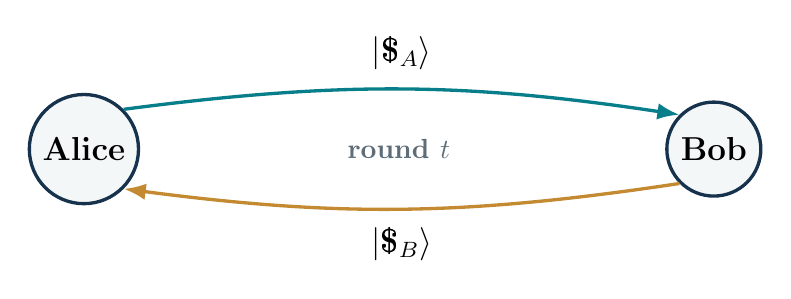
\begin{tikzpicture}[
      >={Latex[length=2.8mm]},
      party/.style={draw=QFEInk,fill=QFEFog,circle,minimum size=1.18cm,
        very thick,font=\large\bfseries},
      atop/.style={->,very thick,draw=QFETeal},
      btop/.style={->,very thick,draw=QFEGold!85!black}
    ]
    \node[party] (alice) at (-4.0,0) {Alice};
    \node[party] (bob) at (4.0,0) {Bob};
    \node[font=\normalsize\bfseries,text=QFEMuted] at (0,0) {round $t$};
    \draw[atop] (alice.north east) to[bend left=8]
      node[above=3pt,font=\large\bfseries] {\qasset{A}}
      (bob.north west);
    \draw[btop] (bob.south west) to[bend left=8]
      node[below=3pt,font=\large\bfseries] {\qasset{B}}
      (alice.south east);
  \end{tikzpicture}

  \vspace{0.55em}
  {\Large Choose $t^*\leftarrow\{1,\ldots,T\}$ at random.\par}

  \vspace{0.35em}
  {\LARGE\bfseries\color{QFETeal}
    $\Pr[t^*=t]=1/T$.\par}

  \note{
    \footnotesize
    \begin{itemize}
      \item This is explicitly an intuition slide. A general protocol need not send raw input registers or have one sharp exchange round.
      \item In the sharp cartoon, choosing the exchange round costs probability $1/T$.
      \item Formally, the proof uses same/adjacent stopping experiments and obtains a mismatch of order $1/T$ by averaging. Do not charge a second random-guess loss on top of that.
      \item Keep all of that bookkeeping out of the audience-facing story.
    \end{itemize}
  }
\end{frame}

\begin{frame}{The Reduction}
  \centering
  {\normalsize At round $t^*$, deliver Alice's message to Bob and withhold
    Bob's message from Alice.\par}

  \vspace{0.20em}
  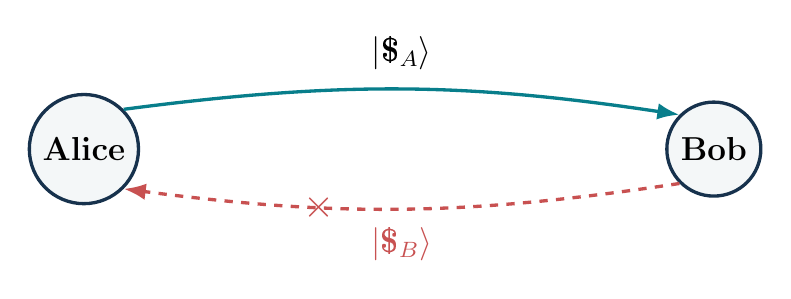
\begin{tikzpicture}[
      >={Latex[length=2.8mm]},
      party/.style={draw=QFEInk,fill=QFEFog,circle,minimum size=1.15cm,
        very thick,font=\large\bfseries},
      delivered/.style={->,very thick,draw=QFETeal},
      withheld/.style={->,very thick,dashed,draw=QFECoral}
    ]
    \node[party] (alice) at (-4.0,0) {Alice};
    \node[party] (bob) at (4.0,0) {Bob};
    \draw[delivered] (alice.north east) to[bend left=8]
      node[above=3pt,font=\large\bfseries] {\qasset{A}}
      (bob.north west);
    \draw[withheld] (bob.south west) to[bend left=8]
      node[pos=0.66,font=\Large,text=QFECoral] {$\times$}
      node[below=3pt,font=\large\bfseries,text=QFECoral]
        {\qasset{B}}
      (alice.south east);
  \end{tikzpicture}

  \vspace{0.05em}
  \begin{columns}[T,onlytextwidth]
    \column{0.47\textwidth}
      \centering
      {\large If Alice rejects, fairness must restore $\qasset{A}$.\par}
    \column{0.47\textwidth}
      \centering
      {\large Bob accepts $\qasset{A}$.\par}
  \end{columns}

  \vspace{0.25em}
  \questionbox{\textbf{No recovery} $\Rightarrow$ unfair.\qquad
    \textbf{Recovery} $\Rightarrow$ two copies of \qasset{A}.}

  \note{
    \footnotesize
    \begin{itemize}
      \item This is the operational cartoon. The arrows need not literally be raw input registers.
      \item Because the TTP holds only bits, the reduction can copy those bits before round $t^*$ and let the two stopping experiments finish separately.
      \item If Bob accepts, he has Alice's identified input. If Alice rejects, input-preserving fairness must return that same identified input to her.
      \item If Alice receives nothing, fairness is already broken. If she receives her input back, the two outputs constitute a clone.
      \item Formally, same-cut and adjacent-cut cases show that one of the $T$ locations produces this mismatch with probability $\Omega(1/T)$.
      \item No quantum register is copied as an intermediate step; the contradiction is at the two final outputs.
    \end{itemize}
  }
\end{frame}

% -----------------------------------------------------------------------------
% 14. Transition from the impossibility result to the candidate construction
% -----------------------------------------------------------------------------

\begin{frame}{Feasibility: What We Show}
  \small
  {\normalsize We have a protocol that satisfies:\par}
  \vspace{0.35em}
  \begin{columns}[T,onlytextwidth]
    \column{0.61\textwidth}
      \uncover<1->{
        {\large\bfseries\color{QFETeal}Property-based security\par}
        \vspace{0.45em}
        {\large\bfseries Correctness\par}
        \vspace{0.15em}
        If both parties are honest, they accept and receive each other's states.
      }

      \uncover<2->{
        \vspace{0.85em}
        {\large\bfseries Soundness\par}
        \vspace{0.15em}
        An honest party leaves with a valid state:
        \[
          \begin{aligned}
            \acclabel&\ \Longrightarrow\ \text{the other party's input},\\
            \rejlabel&\ \Longrightarrow\ \text{its own input}.
          \end{aligned}
        \]
      }

    \column{0.34\textwidth}
      \uncover<3->{
        {\large\bfseries\color{QFEGold!75!black}Still in progress\par}
        \vspace{0.45em}
        Composable security.
      }
  \end{columns}

  \note{
    \footnotesize
    \begin{itemize}
      \item This is the bridge from the impossibility result to the candidate construction: allowing the TTP to hold quantum states removes the copyable-classical-state step.
      \item Formally, both guarantees hold except with negligible probability. On accept, the honest party's output is accepted by the other party's verifier; on reject, it is accepted by its own verifier.
      \item The active manuscript currently contains a proof sketch for these property-based guarantees. Several protocol details and the full proof are still being finalized.
      \item Simulation-based security that composes is future work. Do not claim a particular composable framework yet.
      \item Transition: what changes when the trusted party can actually hold quantum information? Show the whole construction in two pictures before unpacking the machinery.
    \end{itemize}
  }
\end{frame}

% -----------------------------------------------------------------------------
% 15--16. Protocol sketch: what the background must enable
% -----------------------------------------------------------------------------

\begin{frame}{Protocol Sketch I: Input Encoding}
  \centering
  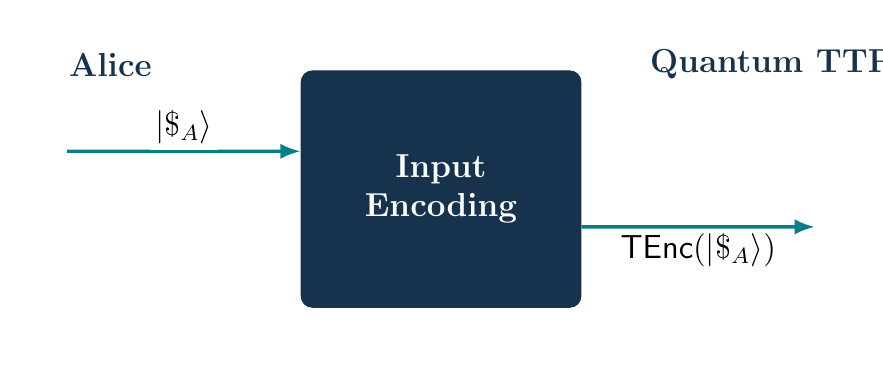
\begin{tikzpicture}[
      >={Latex[length=2.6mm]},
      flow/.style={->,very thick,draw=QFETeal},
      party/.style={font=\large\bfseries,text=QFEInk},
      arrowlabel/.style={font=\large,fill=white,inner sep=2pt},
      function/.style={draw=QFEInk,fill=QFEInk,rounded corners=4pt,
        minimum width=3.55cm,minimum height=3.00cm,align=center,
        text=white,font=\large\bfseries}
    ]
    \path[use as bounding box] (-5.25,-2.05) rectangle (5.25,2.05);
    \node[party] at (-4.20,1.58) {Alice};
    \node[party,align=center] at (4.20,1.58) {Quantum TTP};
    \node[function] (encoding) at (0,0) {Input\\Encoding};
    \draw[flow] (-4.75,0.48) --
      node[arrowlabel,above] {$\qasset{A}$}
      ([yshift=0.48cm]encoding.west);
    \draw[flow] ([yshift=-0.48cm]encoding.east) --
      node[arrowlabel,below] {$\mathsf{TEnc}(\qasset{A})$}
      (4.75,-0.48);
  \end{tikzpicture}

  \note{
    \footnotesize
    \begin{itemize}
      \item This is a roadmap, not notation the audience is expected to know yet. For now, read $\mathsf{TEnc}$ as ``protected encoding''; the next background slides unpack it.
      \item The symbol is deliberately schematic. In the concrete protocol, the TTP holds a QEC-encoded, one-time-padded state; fresh hidden tests are inserted during evaluation rather than stored permanently with it.
      \item Alice has teleported her unique input into that register and keeps no backup copy.
      \item The next cartoon asks how Bob can verify that input without ever receiving it unprotected.
    \end{itemize}
  }
\end{frame}

\begin{frame}{Protocol Sketch II: Verified Evaluation}
  \centering
  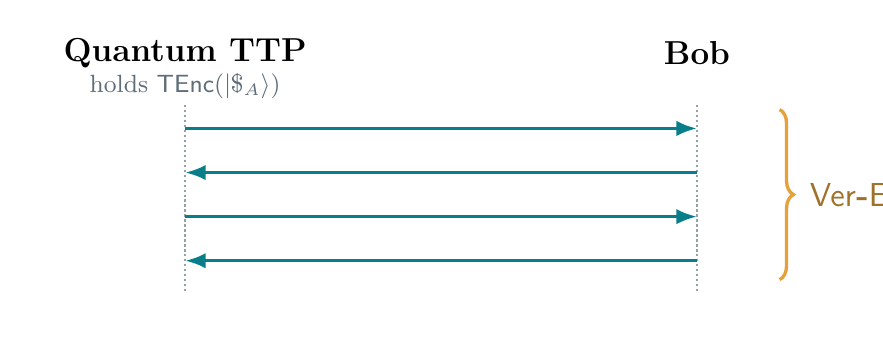
\begin{tikzpicture}[
      >={Latex[length=2.6mm]},
      lane/.style={densely dotted,thick,draw=QFEMuted!65},
      flow/.style={->,very thick,draw=QFETeal}
    ]
    \path[use as bounding box] (-5.25,-1.85) rectangle (5.25,1.90);
    \node[font=\large\bfseries] at (-3.25,1.58) {Quantum TTP};
    \node[font=\large\bfseries] at (3.25,1.58) {Bob};
    \node[font=\small,text=QFEMuted] at (-3.25,1.15)
      {holds $\mathsf{TEnc}(\qasset{A})$};
    \draw[lane] (-3.25,0.92) -- (-3.25,-1.48);
    \draw[lane] (3.25,0.92) -- (3.25,-1.48);
    \draw[flow] (-3.25,0.62) -- (3.25,0.62);
    \draw[flow] (3.25,0.06) -- (-3.25,0.06);
    \draw[flow] (-3.25,-0.50) -- (3.25,-0.50);
    \draw[flow] (3.25,-1.06) -- (-3.25,-1.06);
    \draw[decorate,decoration={brace,amplitude=5pt},very thick,draw=QFEGold]
      (4.30,0.86) -- (4.30,-1.30)
      node[midway,right=7pt,font=\large\bfseries,text=QFEGold!70!black]
      {$\mathsf{Ver\text{-}Eval}$};
  \end{tikzpicture}

  \vspace{0.35em}
  {\large\bfseries
    Catch a cheating Bob before the encoded state is damaged beyond repair.\par}

  \note{
    \footnotesize
    \begin{itemize}
      \item $\mathsf{Ver\text{-}Eval}$ is only a name for the repeated protected interaction in this roadmap; it is not a standard primitive, and the four arrows are not yet the exact messages.
      \item The intended effect is to evaluate Alice's public verifier while interleaving checks, so a cheating Bob is caught before accumulated damage exceeds the correction budget.
      \item The two-party picture is only intuition. The actual checked-gate protocol is three-party: Alice checks Bob's work, and the roles reverse for Bob's input.
      \item Transition: the sketch asks for error correction, hidden tests, and computation that preserves those tests. Build those ingredients next.
    \end{itemize}
  }
\end{frame}

% -----------------------------------------------------------------------------
% 17--23. Background
% -----------------------------------------------------------------------------

\begin{frame}{Background: Quantum Error Correction}
  \centering
  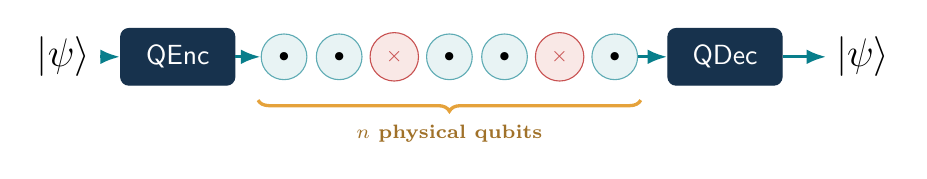
\begin{tikzpicture}[
      >={Latex[length=2.5mm]},
      flow/.style={->,very thick,draw=QFETeal},
      process/.style={draw=QFEInk,fill=QFEInk,rounded corners=3pt,
        text=white,minimum width=1.45cm,minimum height=0.72cm,font=\bfseries},
      qubit/.style={draw=QFETeal!65,fill=QFEPale,circle,
        minimum size=0.58cm,font=\scriptsize\bfseries}
    ]
    \node[font=\Large] (in) at (-5.15,0.65) {$\ket\psi$};
    \node[process] (enc) at (-3.70,0.65) {$\mathsf{QEnc}$};
    \draw[flow] (in) -- (enc);

    \foreach \x/\name in {-2.35/q1,-1.65/q2,-0.95/q3,-0.25/q4,0.45/q5,1.15/q6,1.85/q7} {
      \node[qubit] (\name) at (\x,0.65) {$\bullet$};
    }
    \draw[flow] (enc) -- (q1);
    \node[qubit,draw=QFECoral,fill=QFECoralPale,text=QFECoral] at (-0.95,0.65) {$\times$};
    \node[qubit,draw=QFECoral,fill=QFECoralPale,text=QFECoral] at (1.15,0.65) {$\times$};

    \node[process] (dec) at (3.25,0.65) {$\mathsf{QDec}$};
    \node[font=\Large] (out) at (5.00,0.65) {$\ket\psi$};
    \draw[flow] (q7) -- (dec);
    \draw[flow] (dec) -- (out);

    \draw[decorate,decoration={brace,mirror,amplitude=4pt},very thick,draw=QFEGold]
      (-2.68,0.10) -- (2.18,0.10)
      node[midway,below=5pt,font=\scriptsize\bfseries,text=QFEGold!70!black]
      {$n$ physical qubits};
  \end{tikzpicture}

  \vspace{0.5em}
  \begin{exampleblock}{Correct up to $\lambda$ damaged positions per block}
    \centering
    $\displaystyle
      \bigl(\mathsf{QDec}\circ
        \textcolor{QFECoral}{\mathcal A}\circ\mathsf{QEnc}\bigr)\ket\psi
      =\ket\psi
      \quad\text{if $\mathcal A$ damages at most $\lambda$ positions.}$
  \end{exampleblock}

  \note{
    \footnotesize
    \begin{itemize}
      \item This is the first promised ingredient: it makes ``damaged beyond repair'' precise by giving each encoded block a correction budget.
      \item Keep this at the one-idea level: encode one logical qubit into an entangled block of $n$ physical qubits. In the manuscript, $n=\ell_{\mathrm{code}}$.
      \item Emphasize that this is not cloning. No individual physical qubit contains a copy of the unknown input.
      \item The visible slide suppresses code distance and calls the required correction budget $\lambda$. The active fair-exchange draft actually asks for a code correcting a constant multiple of the security parameter.
      \item $\mathcal A$ denotes the attack/noise channel. The displayed guarantee applies when its effect is supported on at most $\lambda$ physical positions in the block.
      \item Strictly, channels act on density operators; the ket equation is the talk's pure-state shorthand.
      \item Authentication will detect adversarial tampering; QEC repairs the bounded residual damage.
    \end{itemize}
  }
\end{frame}

\begin{frame}{Transversal operations}
  \small
  \begin{columns}[c,onlytextwidth]
    \column{0.65\textwidth}
      \centering
      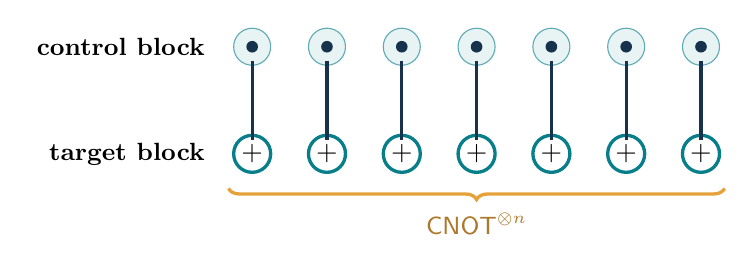
\begin{tikzpicture}[
          qubit/.style={draw=QFETeal!65,fill=QFEPale,circle,
            minimum size=0.47cm,inner sep=0pt},
          target/.style={draw=QFETeal,fill=white,circle,very thick,
            minimum size=0.47cm,inner sep=0pt}
        ]
        \node[font=\small\bfseries,anchor=east] at (-3.28,0.68)
          {control block};
        \node[font=\small\bfseries,anchor=east] at (-3.28,-0.68)
          {target block};
        \foreach \x in {-2.8,-1.85,-0.90,0.05,1.00,1.95,2.90} {
          \node[qubit] at (\x,0.68) {};
          \node[target] at (\x,-0.68) {$+$};
          \fill[QFEInk] (\x,0.68) circle (2.1pt);
          \draw[very thick,draw=QFEInk] (\x,0.50) -- (\x,-0.50);
        }
        \draw[decorate,decoration={brace,mirror,amplitude=4pt},
          very thick,draw=QFEGold]
          (-3.10,-1.12) -- (3.20,-1.12)
          node[midway,below=5pt,font=\small\bfseries,
            text=QFEGold!75!black] {$\mathsf{CNOT}^{\otimes n}$};
      \end{tikzpicture}

    \column{0.30\textwidth}
      \centering
      {\bfseries CNOT truth table\par}
      \vspace{0.25em}
      \renewcommand{\arraystretch}{1.18}
      \begin{tabular}{cc}
        \toprule
        input & output\\
        \midrule
        $\ket{00}$ & $\ket{00}$\\
        $\ket{01}$ & $\ket{01}$\\
        $\ket{10}$ & $\ket{11}$\\
        $\ket{11}$ & $\ket{10}$\\
        \bottomrule
      \end{tabular}
  \end{columns}

  \vspace{0.45em}
  \centering
  {\large
    $\displaystyle
      \mathsf{CNOT}^{\otimes n}
      \mathsf{QEnc}^{\otimes 2}\ket{\psi,\phi}
      =\mathsf{QEnc}^{\otimes 2}
        \mathsf{CNOT}\ket{\psi,\phi}.$\par}

  \note{
    \footnotesize
    \begin{itemize}
      \item The first bit/qubit is the control. CNOT flips the target precisely when the control is one.
      \item For the self-dual CSS/Steane-family example, applying one physical CNOT between every matching pair implements one logical CNOT between the encoded blocks.
      \item The two logical outputs may be entangled, so do not describe this as two independent output states.
      \item This is a concrete transversal operation. Not every gate is available this simply.
    \end{itemize}
  }
\end{frame}

\begin{frame}{Background: Quantum Authentication}
  \centering
  {\small
    $\mathsf{QAS}=(\mathsf{KeyGen},\mathsf{Enc},\mathsf{VerDec})$\par}
  \vspace{0.15em}
  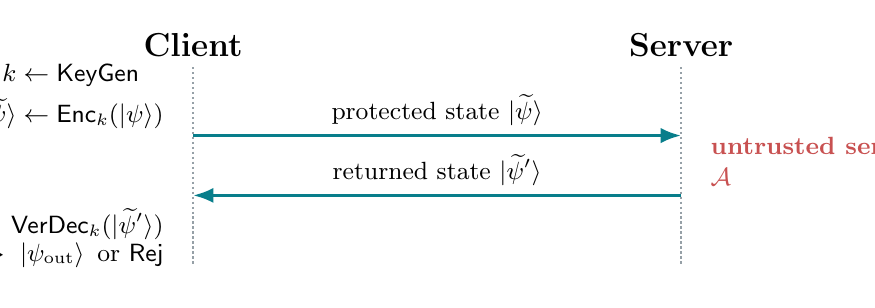
\begin{tikzpicture}[
      >={Latex[length=2.6mm]},
      lane/.style={densely dotted,thick,draw=QFEMuted!65},
      flow/.style={->,very thick,draw=QFETeal}
    ]
    \path[use as bounding box] (-5.2,-1.55) rectangle (5.2,1.65);
    \node[font=\large\bfseries] at (-3.1,1.43) {Client};
    \node[font=\large\bfseries] at (3.1,1.43) {Server};
    \draw[lane] (-3.1,1.15) -- (-3.1,-1.35);
    \draw[lane] (3.1,1.15) -- (3.1,-1.35);

    \node[anchor=east,align=right,font=\small] at (-3.35,0.78)
      {$\begin{aligned}
        k&\leftarrow\mathsf{KeyGen}\\[-0.15em]
        \ket{\widetilde\psi}&\leftarrow\mathsf{Enc}_k(\ket\psi)
      \end{aligned}$};
    \draw[flow] (-3.1,0.28) -- (3.1,0.28)
      node[midway,above=2pt,font=\small,fill=white,inner sep=1pt]
      {protected state $\ket{\widetilde\psi}$};
    \node[anchor=west,align=left,font=\small\bfseries,text=QFECoral]
      at (3.35,-0.05) {untrusted server\\$\mathcal A$};
    \draw[flow] (3.1,-0.48) -- (-3.1,-0.48)
      node[midway,above=2pt,font=\small,fill=white,inner sep=1pt]
      {returned state $\ket{\widetilde\psi'}$};
    \node[anchor=east,align=right,font=\small] at (-3.35,-1.02)
      {$\mathsf{VerDec}_k(\ket{\widetilde\psi'})$\\[-0.1em]
       $\mapsto\ \ket{\psi_{\mathrm{out}}}\ \text{or}\ \rejlabel$};
  \end{tikzpicture}

  \vspace{0.20em}
  \[
    \textbf{Security:}\quad
    \mathsf{Accept}\quad\Longrightarrow\quad
    \ket{\psi_{\mathrm{out}}}\approx\ket\psi.
  \]
  \note{
    \footnotesize
    \begin{itemize}
      \item This is the detection ingredient behind the checks in $\mathsf{Ver\text{-}Eval}$: QEC repairs bounded damage, while authentication detects tampering.
      \item This is the integrity game. The visible slide uses pure states throughout for the audience; a full definition also preserves entanglement with an external reference system.
      \item Here $\mathsf{Enc}$ means authenticated encoding, not encryption for secrecy alone.
      \item The attacker can always destroy the authenticated state and force rejection. Authentication prevents an undetected change.
      \item The authenticating key also commonly hides the plaintext, but privacy is not the conceptual point of this slide.
      \item Transition: the trap code is a concrete way to implement this game.
    \end{itemize}
  }
\end{frame}

\begin{frame}{Background: The Trap Code}
  \small
  \begin{columns}[T,onlytextwidth]
    \column{0.56\textwidth}
      {\large\bfseries Key generation\par}
      \[
        \pi\ \gets_{\$}\ S_{3n},
        \qquad
        x,z\ \gets_{\$}\ \{0,1\}^{3n}.
      \]

      {\large\bfseries Encryption\par}
      \[
        \mathsf{Enc}_{\pi,x,z}(\ket\psi)
        =X^xZ^z\,\pi\!\left(
          \mathsf{QEnc}\ket\psi
          \otimes\ket{0^n}
          \otimes\ket{+^n}
        \right).
      \]

    \column{0.40\textwidth}
      {\large\bfseries Verified decryption\par}
      \vspace{0.4em}
      \begin{enumerate}
        \item Undo $X^xZ^z$, then $\pi$.
        \item Measure and check the $\ket{0^n}$ and $\ket{+^n}$ traps.
        \item If any test fails: $\rejlabel$.
        \item Otherwise: return $\mathsf{QDec}(\text{data})$.
      \end{enumerate}
  \end{columns}

  \note{
    \scriptsize
    \begin{itemize}
      \item This unpacks the trap-code picture behind the $\mathsf{TEnc}$ shorthand, but remember that our TTP does not keep this full ciphertext at rest.
      \item This is the standard one-block trap-code authentication construction. $S_{3n}$ is the symmetric group and $X^xZ^z$ is a uniformly random $3n$-qubit Pauli pad.
      \item For several plaintext qubits, reuse the same permutation $\pi$ and sample an independent Pauli pad for each block.
      \item Undo the pad and permutation; measure $0$-traps in the computational basis and $+$-traps in the Hadamard basis; decode only if all tests pass.
      \item More precisely, $0$-traps detect $X/Y$ components and $+$-traps detect $Z/Y$ components.
      \item Here $n$ is the QEC blocklength introduced earlier; it may be polynomially larger than the number of errors the code corrects.
      \item This manuscript does not keep a persistent standard trap-code ciphertext at the TTP. It inserts fresh tests in every checked operation.
    \end{itemize}
  }
\end{frame}

\begin{frame}{Background: VQFHE}
  \centering
  {\small
    $\mathsf{VQFHE}=(\mathsf{KeyGen},\mathsf{Enc},\mathsf{Eval},\mathsf{VerDec})$\par}
  \vspace{0.15em}
  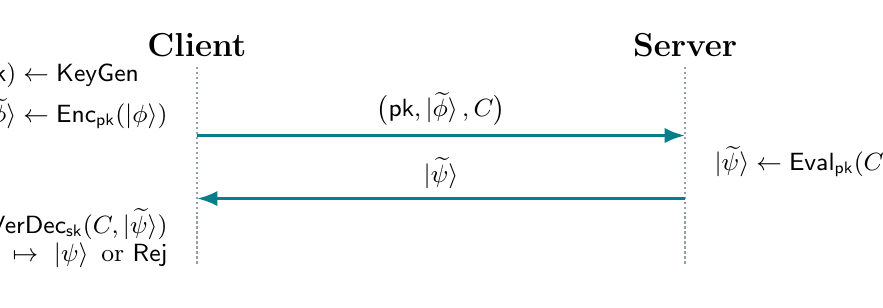
\begin{tikzpicture}[
      >={Latex[length=2.6mm]},
      lane/.style={densely dotted,thick,draw=QFEMuted!65},
      qmsg/.style={->,very thick,draw=QFETeal}
    ]
    \path[use as bounding box] (-5.25,-1.55) rectangle (5.25,1.65);
    \node[font=\large\bfseries] at (-3.1,1.43) {Client};
    \node[font=\large\bfseries] at (3.1,1.43) {Server};
    \draw[lane] (-3.1,1.15) -- (-3.1,-1.35);
    \draw[lane] (3.1,1.15) -- (3.1,-1.35);

    \node[anchor=east,align=right,font=\small] at (-3.35,0.78)
      {$\begin{aligned}
        (\mathsf{pk},\mathsf{sk})&\leftarrow\mathsf{KeyGen}\\[-0.15em]
        \ket{\widetilde\phi}&\leftarrow
          \mathsf{Enc}_{\mathsf{pk}}(\ket\phi)
      \end{aligned}$};
    \draw[qmsg] (-3.1,0.28) -- (3.1,0.28)
      node[midway,above=2pt,font=\small,fill=white,inner sep=1pt]
      {$\bigl(\mathsf{pk},\ket{\widetilde\phi},C\bigr)$};
    \node[anchor=west,align=left,font=\small] at (3.35,-0.05)
      {$\ket{\widetilde\psi}\leftarrow
        \mathsf{Eval}_{\mathsf{pk}}(C,\ket{\widetilde\phi})$};
    \draw[qmsg] (3.1,-0.52) -- (-3.1,-0.52)
      node[midway,above=2pt,font=\small,fill=white,inner sep=1pt]
      {$\ket{\widetilde\psi}$};
    \node[anchor=east,align=right,font=\small] at (-3.35,-1.02)
      {$\mathsf{VerDec}_{\mathsf{sk}}(C,\ket{\widetilde\psi})$\\[-0.1em]
       $\mapsto\ \ket\psi\ \text{or}\ \rejlabel$};
  \end{tikzpicture}

  \vspace{0.45em}
  {\large
    $\displaystyle
      \textbf{Security:}\quad
      \mathsf{Accept}\quad\Longrightarrow\quad
      \ket\psi\approx C\ket\phi.$\par}

  \note{
    \scriptsize
    \begin{itemize}
      \item This is the abstraction behind the $\mathsf{Ver\text{-}Eval}$ roadmap label: compute on a protected state and accept only a certified result.
      \item This is a simplified public-key interface. Read $\mathsf{pk}=(\mathsf{pk}_{\mathrm{enc}},\rho_{\mathrm{evk}})$: encryption uses the classical $\mathsf{pk}_{\mathrm{enc}}$, then the untouched quantum $\rho_{\mathrm{evk}}$ is sent once to the server. It is not freely copyable.
      \item The full syntax may return a separate computation log; here it is folded into $\ket{\widetilde\psi}$, while $C$ remains an input to verified decryption.
      \item The visible pure-state equation is the unitary cartoon. For a general circuit, write $\rho_{\mathrm{out}}\approx\Phi_C(\rho)$ and preserve entanglement with an external reference.
      \item A malicious server may always force rejection. Acceptance certifies the requested computation, up to negligible error.
      \item Privacy is a separate part of the definition: the evaluator should not learn the plaintext.
    \end{itemize}
  }
\end{frame}

\begin{frame}{Background: Homomorphic CNOT}
  \centering
  {\small Both ciphertexts use the \textbf{same hidden permutation} $\pi$.\par}

  \vspace{0.35em}
  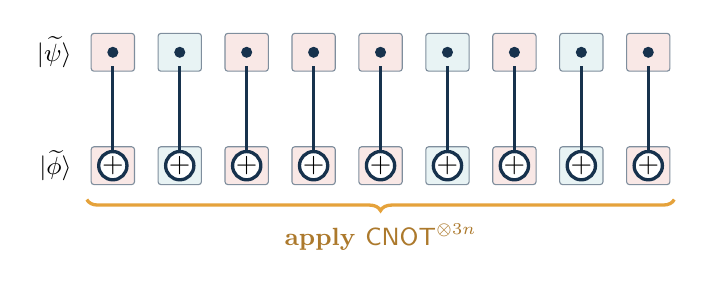
\begin{tikzpicture}[
      cell/.style={draw=QFEInk!55,rounded corners=1pt,
        minimum width=0.55cm,minimum height=0.48cm,inner sep=0pt},
      target/.style={draw=QFEInk,fill=white,circle,very thick,
        minimum size=0.30cm,inner sep=0pt}
    ]
    \node[font=\small\bfseries,anchor=east] at (-4.05,0.72)
      {$\ket{\widetilde\psi}$};
    \node[font=\small\bfseries,anchor=east] at (-4.05,-0.72)
      {$\ket{\widetilde\phi}$};

    \foreach \x/\fillcolor in {
      -3.65/QFECoralPale,-2.80/QFEPale,-1.95/QFECoralPale,
      -1.10/QFECoralPale,-0.25/QFECoralPale,0.60/QFEPale,
      1.45/QFECoralPale,2.30/QFEPale,3.15/QFECoralPale} {
      \node[cell,fill=\fillcolor] at (\x,0.72) {};
      \node[cell,fill=\fillcolor] at (\x,-0.72) {};
      \fill[QFEInk] (\x,0.72) circle (2.0pt);
      \node[target] at (\x,-0.72) {$+$};
      \draw[very thick,draw=QFEInk] (\x,0.54) -- (\x,-0.54);
    }
    \draw[decorate,decoration={brace,mirror,amplitude=4pt},
      very thick,draw=QFEGold]
      (-3.98,-1.15) -- (3.48,-1.15)
      node[midway,below=5pt,font=\small\bfseries,
        text=QFEGold!75!black] {apply $\mathsf{CNOT}^{\otimes 3n}$};
  \end{tikzpicture}

  \vspace{0.55em}
  {\small
    $\displaystyle
      \bigl(\ket{\widetilde\psi'},\ket{\widetilde\phi'}\bigr)
      \leftarrow
      \mathsf{CNOT}^{\otimes 3n}
      \bigl(\ket{\widetilde\psi},\ket{\widetilde\phi}\bigr).$
    \par}

  \note{
    \footnotesize
    \begin{itemize}
      \item This construction visually echoes the transversal-CNOT slide: apply one physical CNOT between every pair of corresponding encrypted positions.
      \item The identical color pattern is only an explanatory view. The evaluator does not know which positions are encoded data, $0$-tests, or $+$-tests.
      \item Both ciphertext blocks share the same secret permutation $\pi$ so that corresponding types line up, but their Pauli pads are sampled independently.
      \item For the first block as control, the hidden Pauli keys update as $(x_1,z_1,x_2,z_2)\mapsto(x_1,z_1\oplus z_2,x_1\oplus x_2,z_2)$. Keep that analysis off the visible construction slide.
    \end{itemize}
  }
\end{frame}

\begin{frame}{Background: Homomorphic CNOT Analysis}
  \footnotesize
  \begin{align*}
    \mathsf{TEnc}_{\pi,Q_1}(\ket\psi)
      &=Q_1\,\pi\!\left(
        \mathsf{QEnc}\ket\psi\otimes\ket{0^n}\otimes\ket{+^n}
      \right),\\[-0.05em]
    \mathsf{TEnc}_{\pi,Q_2}(\ket\phi)
      &=Q_2\,\pi\!\left(
        \mathsf{QEnc}\ket\phi\otimes\ket{0^n}\otimes\ket{+^n}
      \right).
  \end{align*}
  \vspace{-0.35em}
  \centering
  {\footnotesize Same $\pi$; independently random $Q_1,Q_2$.\par}

  \vspace{0.30em}
  \renewcommand{\arraystretch}{1.20}
  \begin{tabularx}{0.97\textwidth}{@{}>{\bfseries}p{0.20\textwidth}X@{}}
    \uncover<2->{new pad keys} &
      \uncover<2->{$\mathsf{CNOT}^{\otimes3n}(Q_1\otimes Q_2)
       =(Q'_1\otimes Q'_2)\mathsf{CNOT}^{\otimes3n}$}\\
    \uncover<3->{same permutation} &
      \uncover<3->{$\mathsf{CNOT}^{\otimes3n}(\pi\otimes\pi)
       =(\pi\otimes\pi)\mathsf{CNOT}^{\otimes3n}$}\\
    \uncover<4->{logical CNOT} &
      \uncover<4->{$\mathsf{CNOT}^{\otimes n}\mathsf{QEnc}^{\otimes2}
       =\mathsf{QEnc}^{\otimes2}\mathsf{CNOT}$}\\
    \uncover<5->{traps unchanged} &
      \uncover<5->{$\mathsf{CNOT}\ket{00}=\ket{00}$,
      \quad $\mathsf{CNOT}\ket{++}=\ket{++}$}
  \end{tabularx}

  \vspace{0.15em}
  \uncover<6->{%
    {\small Universality gets tricky: \cite{alagic-et-al-vqfhe}.\par}%
  }

  \note{
    \footnotesize
    \begin{itemize}
      \item This slide is the analysis of the preceding construction. Read it from top to bottom in the same order as $Q\pi(\cdot)$: pad, permutation, data, traps.
      \item $Q'_1\otimes Q'_2$ is defined by conjugating the original two-block Pauli through $\mathsf{CNOT}^{\otimes3n}$, so the first identity is exact up to the irrelevant Pauli phase.
      \item The second identity is why the two trap-code ciphertexts must share a permutation. Independent permutations would pair data positions with unknown trap types.
      \item CNOT is a clean example, but universality in the cited VQFHE construction is the technically difficult part.
      \item Transition: that was the toolkit. Now instantiate the two idealized protocol pictures, beginning with teleporting the input to the TTP.
    \end{itemize}
  }
\end{frame}

% -----------------------------------------------------------------------------
% 24--29. Candidate construction and resource boundary
% -----------------------------------------------------------------------------

\begin{frame}{Construction I: Input Encoding}
  \centering
  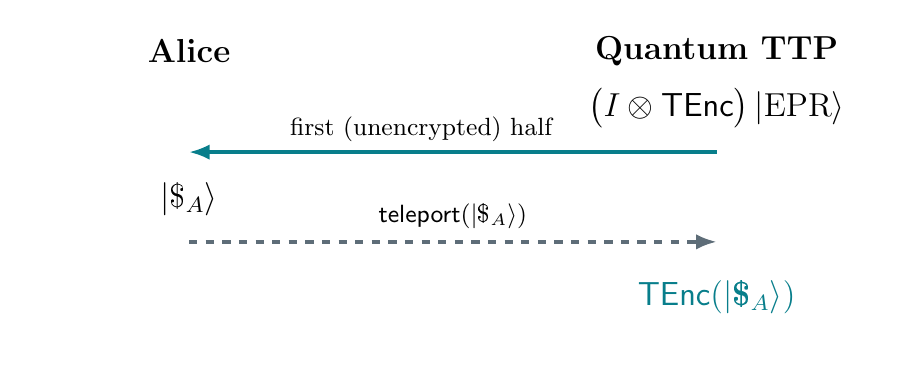
\begin{tikzpicture}[
      >={Latex[length=2.6mm]},
      qmsg/.style={->,very thick,draw=QFETeal},
      cmsg/.style={->,very thick,dashed,draw=QFEMuted}
    ]
    \path[use as bounding box] (-5.40,-1.92) rectangle (5.40,2.00);
    \node[font=\large\bfseries] at (-3.35,1.70) {Alice};
    \node[font=\large\bfseries] at (3.35,1.70) {Quantum TTP};

    \node[font=\large,align=center] at (3.35,0.98)
      {$\bigl(I\otimes\mathsf{TEnc}\bigr)\ket{\mathrm{EPR}}$};
    \draw[qmsg] (3.35,0.42) -- (-3.35,0.42)
      node[pos=0.56,above=2pt,font=\small,fill=white,inner sep=1pt]
      {first (unencrypted) half};
    \node[font=\large] at (-3.35,-0.18) {$\qasset{A}$};
    \draw[cmsg] (-3.35,-0.72) -- (3.35,-0.72)
      node[midway,above=3pt,font=\small,fill=white,inner sep=1pt]
      {$\mathsf{teleport}(\qasset{A})$};
    \node[font=\large\bfseries,text=QFETeal] at (3.35,-1.42)
      {$\mathsf{TEnc}(\qasset{A})$};
  \end{tikzpicture}

  \note{
    \footnotesize
    \begin{itemize}
      \item Back from the background: this realizes Protocol Sketch~I.
      \item The manuscript calls this input commitment; for the talk, simply say that Alice teleports the state to the TTP. It is not a bit-commitment primitive.
      \item The visible $\mathsf{TEnc}$ notation intentionally suppresses the classical teleportation correction and the at-rest QEC-plus-pad distinction.
      \item More precisely, for each teleported input qubit, if the correction is $P_i$, the retained QEC block has pad key $Q_i^0=Q_i^{\mathrm{init}}\overline P_i$. There is no trap permutation in the at-rest state.
      \item Encoded entangled pairs can be prepared before the exchange. During the exchange, the TTP sends one half and updates only a classical one-time-pad key after Alice's teleportation measurement.
      \item Teleportation preserves entanglement with an external reference system.
      \item Next: realize $\mathsf{Ver\text{-}Eval}$ one checked gate at a time.
    \end{itemize}
  }
\end{frame}

% The two Construction-II frames deliberately share one fixed-coordinate
% diagram.  The second is a visual diff: only the coral re-encryption terms
% change.
\newcommand{\checkedgatediagram}[5]{%
  \begin{tikzpicture}[
      >={Latex[length=2.7mm]},
      lane/.style={densely dotted,thick,draw=QFEMuted!65},
      qmsg/.style={->,very thick,draw=QFETeal},
      trapmsg/.style={->,very thick,draw=QFEGold!85!black},
      cmsg/.style={->,very thick,dashed,draw=QFEMuted}
    ]
    \path[use as bounding box] (-5.70,-2.50) rectangle (5.70,1.68);
    \node[font=\large\bfseries] at (-4.75,1.42) {Alice};
    \node[font=\large\bfseries] at (0.25,1.42) {TTP};
    \node[font=\large\bfseries] at (4.15,1.42) {Bob};
    \draw[lane] (-4.75,1.12) -- (-4.75,-2.24);
    \draw[lane] (0.25,1.12) -- (0.25,-1.98);
    \draw[lane] (4.15,1.12) -- (4.15,-2.24);

    \draw[qmsg] (0.25,0.66) -- (4.15,0.66)
      node[pos=0.58,above=3pt,font=\small,fill=white,inner sep=1pt]
      {#1};
    \draw[qmsg] (4.15,-0.02) -- (0.25,-0.02)
      node[midway,above=2pt,font=\small,fill=white,inner sep=1pt]
      {#2};
    \draw[trapmsg] (0.25,-0.78) -- (-4.75,-0.78)
      node[midway,above=3pt,font=\scriptsize,fill=white,inner sep=1pt,align=center]
      {#3\\[-0.1em]#4};
    \draw[cmsg] (-4.75,-1.84) -- (0.25,-1.84)
      node[midway,above=2pt,font=\scriptsize,fill=white,inner sep=1pt,align=center]
      {$o_0\leftarrow\mathsf{Meas}_Z\bigl((G^\dagger)^{\otimes2}\ket{T_0}\bigr)$\\[-0.1em]
       $o_+\leftarrow\mathsf{Meas}_X\bigl((G^\dagger)^{\otimes2}\ket{T_+}\bigr)$};
    \node[font=\scriptsize,align=center] at (0.25,-2.39) {#5};

    \draw[decorate,decoration={brace,amplitude=5pt},very thick,draw=QFEGold]
      (5.12,0.88) -- (5.12,-2.12)
      node[midway,right=6pt,text=QFEGold!70!black,font=\scriptsize\bfseries,align=left]
      {repeat for\\$j=1,\ldots,n$};
  \end{tikzpicture}
}

\begin{frame}{Construction II: Homomorphic Gate Evaluation}
  \centering
  {\scriptsize
    $\ket W:=Q\,\pi_E\bigl(\ket{D_j}\otimes\ket{0^w}\otimes\ket{+^w}\bigr)$,
    \\[-0.05em]
    {\phantom{$\reenc{R\leftarrow\text{fresh Pauli}}$.}}
    \par}

  \vspace{0.08em}
  \checkedgatediagram
    {$\ket W$}
    {$G^{\otimes3}\ket W$}
    {$\ket{T_0}=\pi_0\bigl(GQ_0\ket{0^w},\,GX^u\ket{0^w}\bigr)$}
    {$\ket{T_+}=\pi_+\bigl(GQ_+\ket{+^w},\,GZ^v\ket{+^w}\bigr)$}
    {check $(o_0,o_+)$;\\[-0.1em]
      keep $GQ_D\ket{D_j}$}

  \note{
    \scriptsize
    \begin{itemize}
      \setlength{\itemsep}{0pt}
      \item Warm-up: no fresh re-encryption. This is one complete per-coordinate interaction; the TTP checks before advancing to $j+1$.
      \item $G$ is the current physical gate. The pure-state notation is shorthand: $D_j$ may be entangled with other columns and a reference.
      \item $Q$ is the aggregate pad on the permuted triple: $\pi_E^{-1}Q\pi_E=Q_D\otimes Q_0\otimes Q_+$. Thus the data register is already encrypted by $Q_D$.
      \item Up to phase, write $Q_0\ket{0^w}=X^e\ket{0^w}$ and $Q_+\ket{+^w}=Z^f\ket{+^w}$; these bit strings are needed only for the exact checks in the notes.
      \item Fresh $u,v\in\{0,1\}^w$ and $\pi_0,\pi_+\in S_2$ hide the known-output comparison traps. Alice applies $G^\dagger$, measures the $0$-pair in $Z$ and the $+$-pair in $X$, and returns $(o_0,o_+)$.
      \item Honest expected strings are $(e,u)$ and $(f,v)$. The TTP retains $GQ_D\ket{D_j}$, which represents $G\ket{D_j}$ under the updated pad $Q_{D,\mathrm{new}}=GQ_DG^\dagger$.
      \item This warm-up is not the final construction: without fresh Pauli re-encryption, correlations can persist between calls.
    \end{itemize}
  }
\end{frame}

\begin{frame}{Construction II: Add Re-encryption}
  \centering
  {\scriptsize
    $\ket W:=Q\,\pi_E\bigl(\ket{D_j}\otimes\ket{0^w}\otimes\ket{+^w}\bigr)$,
    \\[-0.05em]
    $\reenc{R\leftarrow\text{fresh Pauli}}$.
    \par}

  \vspace{0.08em}
  \checkedgatediagram
    {$\bigl(\ket W,\reenc{R}\bigr)$}
    {$\reenc{R}\,G^{\otimes3}\ket W$}
    {$\ket{T_0}=\pi_0\bigl(\reenc{R_0}GQ_0\ket{0^w},\,GX^u\ket{0^w}\bigr)$}
    {$\ket{T_+}=\pi_+\bigl(\reenc{R_+}GQ_+\ket{+^w},\,GZ^v\ket{+^w}\bigr)$}
    {check $(o_0,o_+)$;\\[-0.1em]
      keep $\reenc{R_D}GQ_D\ket{D_j}$}

  \note{
    \scriptsize
    \begin{itemize}
      \setlength{\itemsep}{0pt}
      \item Same interaction; coral marks the additions. $R$ is a fresh Pauli on the permuted triple, sent classically. Bob applies $G^{\otimes3}$ and then $R$.
      \item Here $G$ is the current physical gate and $Q$ collects the existing pads. In hidden order, $\pi_E^{-1}R\pi_E=R_D\otimes R_0\otimes R_+$; Bob cannot identify the three roles.
      \item In manuscript notation, $R=P'_{\pi_E}$ and $(R_D,R_0,R_+)=(Q',P'_0,P'_+)$. Independent component Paulis are uniform in $\mathcal P_{3w}$ up to irrelevant phase.
      \item Write $G^\dagger R_sG=X^{a_s}Z^{b_s}$. After applying $\pi_0^{-1},\pi_+^{-1}$ to the outcomes, the expected strings are $(a_0\oplus e,u)$ and $(b_+\oplus f,v)$.
      \item On acceptance the TTP retains $R_DGQ_D\ket{D_j}$, representing $G\ket{D_j}$ under the updated pad $Q_{D,\mathrm{new}}=R_DGQ_DG^\dagger$.
      \item This remains a candidate construction; the coherent-attack and culprit-attribution arguments are still being finalized.
    \end{itemize}
  }
\end{frame}

\begin{frame}{Construction III: Circuit Evaluation}
  \centering
  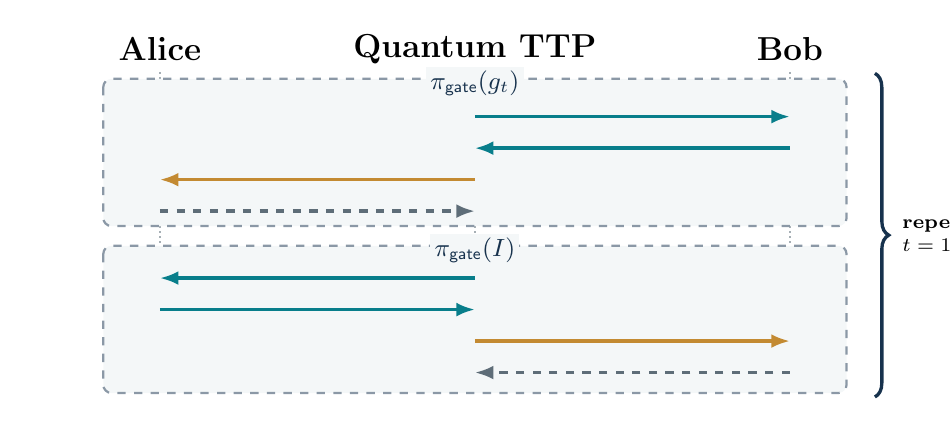
\begin{tikzpicture}[
      >={Latex[length=2.35mm]},
      lane/.style={densely dotted,thick,draw=QFEMuted!55},
      qmsg/.style={->,very thick,draw=QFETeal},
      trapmsg/.style={->,very thick,draw=QFEGold!85!black},
      cmsg/.style={->,very thick,dashed,draw=QFEMuted}
    ]
    \path[use as bounding box] (-5.68,-2.47) rectangle (5.68,2.38);
    \node[font=\large\bfseries] at (-4.00,2.11) {Alice};
    \node[font=\large\bfseries] at (0,2.11) {Quantum TTP};
    \node[font=\large\bfseries] at (4.00,2.11) {Bob};
    \draw[lane] (-4,1.82) -- (-4,-2.25);
    \draw[lane] (0,1.82) -- (0,-2.25);
    \draw[lane] (4,1.82) -- (4,-2.25);

    \draw[draw=QFEInk!50,fill=QFEFog,rounded corners=3pt,dashed,thick]
      (-4.72,1.73) rectangle (4.72,-0.14);
    \node[fill=QFEFog,inner sep=1.5pt,font=\small\bfseries,text=QFEInk]
      at (0,1.67) {$\pi_{\mathsf{gate}}(g_t)$};
    \draw[qmsg] (0,1.25) -- (4,1.25);
    \draw[qmsg] (4,0.85) -- (0,0.85);
    \draw[trapmsg] (0,0.45) -- (-4,0.45);
    \draw[cmsg] (-4,0.05) -- (0,0.05);

    \draw[draw=QFEInk!50,fill=QFEFog,rounded corners=3pt,dashed,thick]
      (-4.72,-0.39) rectangle (4.72,-2.26);
    \node[fill=QFEFog,inner sep=1.5pt,font=\small\bfseries,text=QFEInk]
      at (0,-0.45) {$\pi_{\mathsf{gate}}(I)$};
    \draw[qmsg] (0,-0.80) -- (-4,-0.80);
    \draw[qmsg] (-4,-1.20) -- (0,-1.20);
    \draw[trapmsg] (0,-1.60) -- (4,-1.60);
    \draw[cmsg] (4,-2.00) -- (0,-2.00);

    \draw[decorate,decoration={brace,amplitude=5pt},very thick,draw=QFEInk]
      (5.08,1.80) -- (5.08,-2.31)
      node[midway,right=6pt,font=\scriptsize\bfseries,align=left]
      {repeat for\\$t=1,\ldots,T$};
  \end{tikzpicture}

  \vspace{-0.05em}
  {\small\bfseries\color{QFETeal}
    For each gate, run $\pi_{\mathsf{gate}}$ twice, with Alice and Bob
    exchanging roles.\par}

  \note{
    \scriptsize
    \begin{itemize}
      \item For Alice's input, Alice is the sender and Bob the verifier. Bob evaluates the actual gate and Alice checks; the identity pass reverses their roles.
      \item Show all eight arrows even if the labels are abbreviated; the repeated geometry is the point.
      \item In each four-message call, blue marks the evaluator exchange, gold the trap pair sent to the checker, and dashed gray the classical outcomes.
      \item A circuit is not eight messages total: the pair repeats for every directly supported instruction and each gate call repeats over every physical coordinate.
      \item The identity pass makes both parties serve as evaluator and refreshes the hidden state before the next instruction.
      \item Measurement instructions use a separate trap-checked primitive. Other gate and measurement details in the active rewrite are less polished, so keep the visible claim to one generic circuit step.
      \item This is a candidate construction. The load-bearing coherent-attack security argument is still being finalized; do not present it as a finished theorem.
    \end{itemize}
  }
\end{frame}

\begin{frame}{Construction IV: Full Exchange}
  \centering
  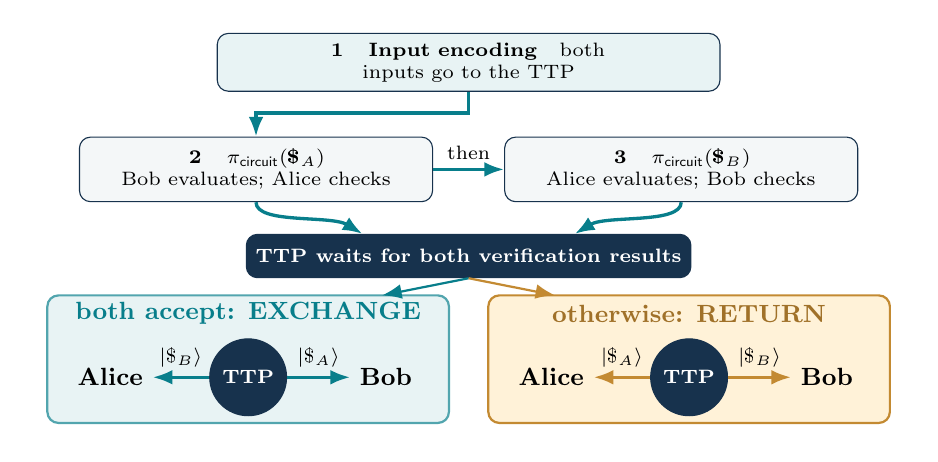
\begin{tikzpicture}[
      >={Latex[length=2.5mm]},
      flow/.style={->,very thick,draw=QFETeal},
      stage/.style={draw=QFEInk,fill=QFEFog,rounded corners=4pt,
        text width=4.25cm,minimum height=0.82cm,align=center,font=\scriptsize},
      decision/.style={draw=QFEInk,fill=QFEInk,rounded corners=4pt,
        minimum width=4.65cm,minimum height=0.55cm,text=white,align=center,font=\scriptsize\bfseries},
      party/.style={font=\small\bfseries}
    ]
    \path[use as bounding box] (-5.60,-2.90) rectangle (5.60,2.26);
    \node[stage,fill=QFEPale,text width=6.15cm,minimum height=0.62cm]
      (encode) at (0,1.82)
      {\textbf{1\quad Input encoding}\quad both inputs go to the TTP};
    \node[stage] (verifya) at (-2.70,0.46)
      {\textbf{2\quad $\pi_{\mathsf{circuit}}(\asset{A})$}\\Bob evaluates; Alice checks};
    \draw[flow] (encode.south) -- ++(0,-0.27) -| (verifya.north);
    \node[stage] (verifyb) at (2.70,0.46)
      {\textbf{3\quad $\pi_{\mathsf{circuit}}(\asset{B})$}\\Alice evaluates; Bob checks};
    \draw[flow] (verifya.east) --
      node[midway,above=2pt,font=\scriptsize,fill=white,inner sep=1pt] {then}
      (verifyb.west);
    \node[decision] (decision) at (0,-0.64)
      {TTP waits for both verification results};
    \draw[flow] (verifya.south)
      .. controls ++(0,-0.28) and ++(-0.40,0.24)
      .. ([xshift=-1.35cm]decision.north);
    \draw[flow] (verifyb.south)
      .. controls ++(0,-0.28) and ++(0.40,0.24)
      .. ([xshift=1.35cm]decision.north);

    \draw[draw=QFETeal!70,fill=QFEPale,rounded corners=4pt,thick]
      (-5.35,-1.14) rectangle (-0.25,-2.76);
    \node[font=\small\bfseries,text=QFETeal] at (-2.80,-1.37)
      {both accept: EXCHANGE};
    \node[party] (as) at (-4.55,-2.18) {Alice};
    \node[draw=QFEInk,fill=QFEInk,circle,text=white,minimum size=0.58cm,font=\scriptsize\bfseries]
      (ts) at (-2.80,-2.18) {TTP};
    \node[party] (bs) at (-1.05,-2.18) {Bob};
    \draw[flow] (ts) -- (as)
      node[midway,above=2pt,font=\scriptsize,fill=QFEPale,inner sep=1pt] {$\qasset{B}$};
    \draw[flow] (ts) -- (bs)
      node[midway,above=2pt,font=\scriptsize,fill=QFEPale,inner sep=1pt] {$\qasset{A}$};

    \draw[draw=QFEGold!85!black,fill=QFEGoldPale,rounded corners=4pt,thick]
      (0.25,-1.14) rectangle (5.35,-2.76);
    \node[font=\small\bfseries,text=QFEGold!70!black] at (2.80,-1.37)
      {otherwise: RETURN};
    \node[party] (af) at (1.05,-2.18) {Alice};
    \node[draw=QFEInk,fill=QFEInk,circle,text=white,minimum size=0.58cm,font=\scriptsize\bfseries]
      (tf) at (2.80,-2.18) {TTP};
    \node[party] (bf) at (4.55,-2.18) {Bob};
    \draw[->,very thick,draw=QFEGold!85!black] (tf) -- (af)
      node[midway,above=2pt,font=\scriptsize,fill=QFEGoldPale,inner sep=1pt] {$\qasset{A}$};
    \draw[->,very thick,draw=QFEGold!85!black] (tf) -- (bf)
      node[midway,above=2pt,font=\scriptsize,fill=QFEGoldPale,inner sep=1pt] {$\qasset{B}$};

    \draw[->,thick,draw=QFETeal] (decision.south) -- (-1.10,-1.14);
    \draw[->,thick,draw=QFEGold!85!black] (decision.south) -- (1.10,-1.14);
  \end{tikzpicture}

  \note{
    \scriptsize
    \begin{itemize}
      \item The two one-sided circuit evaluations leave both processed encrypted input states and their updated pad keys at the TTP until both verification results are known.
      \item On success the outputs cross. On failure each updated input state returns to its original owner.
      \item Bob runs the public circuit that validates Alice's input; Alice runs the circuit validating Bob's.
      \item Steps 2 and 3 are side by side only to save vertical space. The ``then'' arrow indicates the sequential schedule; no parallel-composition claim is being made.
      \item Fairness comes from delayed release: neither party gets the other's unique input before both checks complete.
      \item The quantum resources can be prepared in advance. During the exchange, the TTP's quantum behavior is intended to reduce to storage, communication, and hidden permutations implemented with routing/SWAP; checks and key updates are classical.
      \item This removes the copyable-classical-state step from the impossibility argument: the trusted party now holds irreplaceable quantum states.
      \item Say ``candidate construction'' while the complete security proof and several circuit details remain in progress.
    \end{itemize}
  }
\end{frame}

\begin{frame}{Result: Feasibility with a Quantum TTP}
  \small
  {\large\bfseries\color{QFETeal}
    During pre-processing, the TTP prepares:\par}
  \vspace{0.30em}
  \begin{itemize}
    \setlength{\itemsep}{0.30em}
    \item $(I\otimes\mathsf{TEnc})\ket{\mathrm{EPR}}$ for input encoding;
    \item $\mathsf{TEnc}(\ket0)$ and $\mathsf{TEnc}(\ket{T})$ in the VQFHE
      evaluation key;
    \item $X^x\ket0$ and $Z^z\ket+$ traps for gate evaluation;
    \item $G X^x\ket0$ and $G Z^z\ket+$ traps measured during gate verification.
  \end{itemize}

  \vspace{0.50em}
  \pause
  {\normalsize \textbf{Online:} quantum storage and communication; routing uses
    only \textbf{SWAP gates}.\\[0.15em]
    Checks and key updates are classical.\par}

  \note{
    \scriptsize
    \begin{itemize}
      \setlength{\itemsep}{0pt}
      \item This restates the feasibility result as a resource theorem: every listed quantum state is input-independent and can be prepared before Alice or Bob supplies an input.
      \item The visible $\mathsf{TEnc}$ in the first bullet is the same schematic shorthand used earlier. The actual retained halves are QEC encoded and one-time padded; teleportation moves the inputs into them.
      \item The second bullet is audience-level shorthand for protected auxiliary inputs in the VQFHE evaluation key. It is not a claim that $\ket0$ and $\ket+$ alone are a complete universal evaluation key; the exact construction includes additional gate-dependent resources.
      \item The last two visible bullets are the two pairs in a checked-gate call: evaluator traps and fresh known-output traps for the verifier's measurements. Their pads are independent; repeated $x,z$ is schematic. A separate checked computational-basis measurement uses a fresh $X^r\ket0$ trap.
      \item The TTP also keeps classical one-time-pad keys, secret permutations, and expected test outcomes.
      \item Online, the TTP stores and communicates quantum registers. Its routing operations can be implemented with SWAP gates; the tests and one-time-pad updates are classical.
      \item Say ``candidate theorem'': the current manuscript has the construction and a proof sketch, while the complete security proof and some circuit details remain in progress.
    \end{itemize}
  }
\end{frame}

% Avoid asking the full-width progress bar to extend past the final frame's
% title box; the closing and backup pages do not need it.
\metroset{progressbar=none}

\begin{frame}{Thank You}
  \centering
  \vfill
  {\Huge\bfseries\color{QFETeal}Questions?\par}
  \vfill

  \note{
    Stop here for questions. The references that follow are backup pages.
  }
\end{frame}

% Bibliography is an unnumbered backup frame rather than part of the timed talk.
\begin{frame}[allowframebreaks,noframenumbering]{References}
  \scriptsize
  \printbibliography[heading=none]
\end{frame}

\end{document}
